\documentclass[10pt,twoside,a4paper]{article}

\title{Resume}

\date{2019-4-14}

\author{Junaid Shaikh}

\usepackage{multicol}
\usepackage{hyperref}
\usepackage{graphicx}
\usepackage[margin=0.7in] {geometry}


\begin{document}


\begin{center}

%Name to be align in center

	{\scshape \LARGE Junaid Shaikh}

	\line(1,0){250}

\end{center}



%giving no indentation to address
\begin{multicols}{2}

%address
\noindent
406,\\
Sonigara Opal,\\
Near Bombay Selection,\\
Old Mumbai-Pune Highway,\\
Chinchwad, \\
Pune 411019 \\
\columnbreak

%contact details to the right

\begin{flushright}
Contact: +91 7773973999\\
e-mail:	junaidlatur@gmail.com\\
Git-Hub: 	\url{https://github.com/Junaid7000}\\
\end{flushright}
\end{multicols}



%to add image 

\begin{flushright}
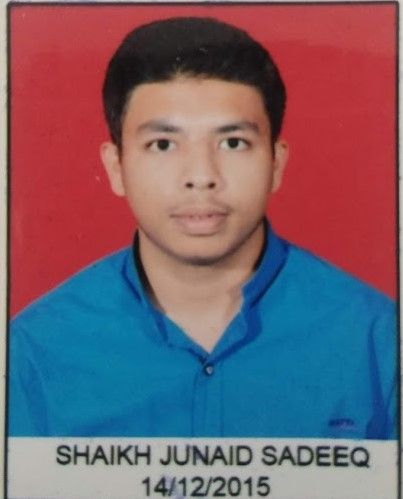
\includegraphics[width=20mm]{img.jpg}
\end{flushright}

% body start
\noindent
\textbf{Career Objective:}

To seek a challenging position as a Machine Learning Engineer with an organization of repute, where I can utilize my skills and knowledge of mechanical engineering concepts and advance technologies like Deep learning, image processing.\\

%table for educational background
\noindent
\textbf{Education:}
\begin{center}
\begin{tabular}{|c|c|c|c|c|}
\hline
Degree & College/School & University/Board & Passing Year & Pass Percentage \\
\hline
S.S.C. & S.V.M.V Latur & Latur Board & 2014 & 94.80 \\
\hline
H.S.C. & DSC Latur & Latur Board & 2016 & 80.31 \\
\hline
First Year & PCCoE, pune & SPPU, Pune & 2017 & 82.016 \\
\hline
Second Year & PCCoE, pune & SPPU, Pune & 2018 & 72.16 \\
\hline
\end{tabular}
\\
\end{center}


\noindent
\textbf{Projects:} 
%numerated list 
\begin{enumerate}
\item e-Yantra Project Based Competition: Project on Animal home coming. Where animals and Habitates are extracted from image and than image is feed to deep learning model which classifies the animal and maps the animal to there habitate. This data is later transfered to a bot which searches the minimum path for reaching to animal, Pick the animal and place it in respective habitate.
\item Parking sensor for vehicle using Arduino uno.
\item Project related to calculating brake power and efficiency of IC engine.
\item Water Level indicator using arduino uno.
\item All terrain bot using Arduino uno.
\item Lane detection for self-driving car using OpenCV.
\item  Deep learning project to classify given images of digits and alphabets.
\item Hand gesture recognition using deep learning
\\
\end{enumerate}

%Training and internship details
\noindent
\textbf{Training and Internship:}
\begin{itemize}
\item Project based Learning By Eyantra,IIT Bombay.
\item Hands On Training For Deep Learning using Tensorflow by IBM.
\item Hands On Training For Android by Skylabs and IIT hyderabad.
\item Artifical Intelligence and Machine Learning Workshop At PCCOE, Pune. 
\item Hands on Training on core Java  
\end{itemize}

%Research Publication details
\noindent
\textbf{Research Publication:}
None\\

\newpage
%Soft skills
\noindent
\textbf{Soft Skills}
\begin{enumerate}
\item Persistant
\item Problem Solving
\item Responsibility
\item Communication
\item Leadership
\item Positive attitude
\item Team Work 
\\
\end{enumerate}

%co-curricular Activity
\noindent
\textbf{Co-Curricular Activity}
\begin{itemize}
\item Secured 2nd place at Machine-Learing competition at PICT
\item Secured 3rd place at All terrian bot competition at PCCOE 
\item Recipient of Pytorch Scholarship by Facebook and Udacity
\item Recipient of Google India Android challenge by Google and Udacity
\item Completed Coursera Machine Learning course By Andrew NG.
\end{itemize}

















\end{document}
